\documentclass[rgb]{beamer}

\usepackage[english]{babel}
\usepackage[utf8]{inputenc}
\usepackage{xcolor}
\usepackage{listings}
\usepackage{adjustbox}
\usepackage{amsmath}
\usepackage{multirow}
\usepackage[linewidth=1pt]{mdframed}

% Graphics
\usepackage{graphicx}

\usepackage{tikz}
\usetikzlibrary{calc,shapes.multipart,chains,arrows}

% Font
\usepackage{paratype}
\setbeamerfont{frametitle}{family=\bf}

% Beamer theme settings
\usecolortheme{seagull}
\setbeamertemplate{itemize item}{\raisebox{0.8mm}{\rule{1.8mm}{1.2mm}}}
\usenavigationsymbolstemplate{} % no navigation buttons

\usepackage{listings}

% Define Language
\lstdefinelanguage{fsharp}
{
  % list of keywords
  morekeywords={
    and,
    do,
    else,
    exception,
    for,
    fun,
    function,
    if,
    in,
    let,
    match,
    module,
    mutable,
    open,
    of,
    rec,
    then,
    try,
    type,
    unsafe,
    use,
    val,
    when,
    while,
    with,
  },
  sensitive=true, % keywords are not case-sensitive
  morecomment=[l]{//}, % l is for line comment
%  otherkeywords={>,<,=,<=,>=,!,*,/,-,+,|,&,||,&&,==,=>},
  morestring=[b]" % defines that strings are enclosed in double quotes
}

% Define Colors
\usepackage{color}
\definecolor{eclipseBlue}{RGB}{42,0.0,255}
\definecolor{eclipseGreen}{RGB}{63,127,95}
\definecolor{eclipsePurple}{RGB}{127,0,85}

\newcommand{\fop}[1]{\mbox{\ttfamily\color{eclipseBlue}#1}}
\newcommand{\fw}[1]{\mbox{\ttfamily\bfseries\color{eclipsePurple}#1}}

% Set Language
\lstset{
  language={fsharp},
  basicstyle=\ttfamily, % Global Code Style
  captionpos=b, % Position of the Caption (t for top, b for bottom)
  extendedchars=true, % Allows 256 instead of 128 ASCII characters
  tabsize=2, % number of spaces indented when discovering a tab
  columns=fixed, % make all characters equal width
  keepspaces=true, % does not ignore spaces to fit width, convert tabs to spaces
  showstringspaces=false, % lets spaces in strings appear as real spaces
  breaklines=true, % wrap lines if they don't fit
  frame=trbl, % draw a frame at the top, right, left and bottom of the listing
  frameround=tttt, % make the frame round at all four corners
  framesep=4pt, % quarter circle size of the round corners
  numbers=left, % show line numbers at the left
  numberstyle=\small\ttfamily, % style of the line numbers
  commentstyle=\slshape\bfseries\color{eclipseGreen}, % style of comments
  keywordstyle=\bfseries\color{eclipsePurple}, % style of keywords
  stringstyle=\color{eclipseBlue}, % style of strings
  emph=[1] {
    false,
    true,
    Set,
    Map,
    List,
    ImgUtil,
    Pegs,
    String,
    Array,
    Array2D
  },
  emphstyle=[1]{\color{eclipseBlue}},
  moredelim=**[is][\color{red}]{@@}{@@}
}

\newcommand{\theyear}{2020}
\newcommand{\sem}[1]{[\![#1]\!]}
\newcommand{\seme}[1]{\sem{#1}\varepsilon}
\newcommand{\semzero}[1]{\sem{#1}_0}

\newcommand{\emptymap}{\{\}}
\newcommand{\fracc}[2]{\begin{eqnarray} \frac{\begin{array}{c} #1
    \end{array}}{\begin{array}{c} #2 \end{array}} \end{eqnarray}}
\newcommand{\sembox}[1]{\hfill \normalfont \mbox{\fbox{\(#1\)}}}
\newcommand{\sempart}[2]{\subsubsection*{\rm\em #1 \sembox{#2}}}
\newcommand{\axiom}[1]{\begin{eqnarray} \begin{array}{c} #1 \end{array} \end{eqnarray}}
\newcommand{\fraccn}[2]{\refstepcounter{equation}\mbox{$\frac{\begin{array}{c} #1 \end{array}}{\begin{array}{c} #2 \end{array}}$}~(\arabic{equation})}
\newcommand{\fraccc}[2]{\mbox{$\frac{\begin{array}{c} #1 \end{array}}{\begin{array}{c} #2 \end{array}}$}}
\newcommand{\onepart}[1]{\noindent\hfill#1\hfill~\vspace{2mm}}
\newcommand{\twopart}[2]{\noindent\hfill#1\hfill#2\hfill~\vspace{2mm}}
\newcommand{\threepart}[3]{\noindent\hfill#1\hfill#2\hfill#3\hfill~\vspace{2mm}}
%\newcommand{\axiomm}[1]{\refstepcounter{equation}\mbox{$\begin{array}{c} #1 \end{array}$}~(\arabic{equation})}
\newcommand{\axiomm}[1]{$\begin{array}{c} #1 \end{array}$}
%\newcommand{\ar}[1]{\stackrel{#1}{\longrightarrow}}
\newcommand{\vd}{\vdash}
\newcommand{\Ran}{{\rm Ran}}
\newcommand{\Dom}{{\rm Dom}}
\newcommand{\kw}[1]{\texttt{#1}}
\newcommand{\id}[1]{\mbox{\it{#1}}}
\newcommand{\rarr}{\rightarrow}
\newcommand{\eval}{\rarr}
\newcommand{\evals}{\leadsto}
\newcommand{\larr}{\leftarrow}

\newcommand{\head}[1]{\vspace{3mm} \textbf{\normalsize #1}}
\newcommand{\headsp}[1]{\head{#1}\vspace{1ex}}
\newcommand{\size}{\ensuremath{\mathrm{size}}}
\renewcommand{\log}{\ensuremath{\mathrm{log}}}

\newcommand{\setallthemecolors}[1]{%
\setbeamercolor*{palette primary}{use=structure,fg=white,bg=#1}%
\setbeamercolor*{palette secondary}{use=structure,fg=white,bg=#1}%
\setbeamercolor*{palette tertiary}{use=structure,fg=white,bg=#1}}

\definecolor{black}{RGB}{0,0,0}
\definecolor{maroon}{RGB}{128,0,0}
\definecolor{olive}{RGB}{128,128,0}
\definecolor{green}{RGB}{0,128,0}
\definecolor{purple}{RGB}{128,0,128}
\definecolor{teal}{RGB}{0,128,128}
\definecolor{darkteal}{RGB}{0,92,92}
\definecolor{navy}{RGB}{0,0,128}
\definecolor{gray}{RGB}{128,128,128}
\definecolor{darkgray}{RGB}{60,60,60}
\definecolor{darkred}{RGB}{139,0,0}

%palette

% #173F5F (dark blue)
\definecolor{darkblue}{RGB}{23,63,95}
% #20639B (blue)
\definecolor{blue}{RGB}{32,99,155}
% #3CAEA3 (green)
\definecolor{magenta}{RGB}{60,174,163}
% #F6D55C (yellow)
\definecolor{yellow}{RGB}{246,213,92}
% #ED553B (red)
\definecolor{red}{RGB}{237,85,59}


\usecolortheme{whale}
\useoutertheme{infolines}
\useinnertheme{rectangles}

\newcommand{\popsettitle}[2]{%
\setallthemecolors{#1}%
\newcommand{\popemne}{#2}%
\title{Programmering og Problemløsning}%
\subtitle{#2}%
\author{Martin Elsman}%
\date{}%
\institute[DIKU]{Datalogisk Institut, Københavns Universitet (DIKU)}}

\newcommand{\popmaketitleframe}{%
  \frame{\titlepage%
   \vspace{-15mm}%
   \par\noindent\rule{\textwidth}{0.4pt}%

   \vspace{4mm}%
   \tableofcontents%
   \vspace{-4mm}%
   \par\noindent\rule{\textwidth}{0.4pt}%
  }%
  \section*{\popemne}%
}


\popsettitle{blue}{Rekursion (Del 2)}  % see ../util.tex for colors

\begin{document}

\popmaketitleframe

%%%%%%%%%%%%%%%%%%%%%%%%%%%%%%%%%%%%%%%%%%%%%%%%
\subsection{Pattern-matching på lister}
%%%%%%%%%%%%%%%%%%%%%%%%%%%%%%%%%%%%%%%%%%%%%%%%

\begin{frame}[fragile]
\begin{footnotesize}
  \headsp{Konstruktion af lister}

  Lister er opbygget af listekonstruktørerne:
\begin{lstlisting}[numbers=none,frame=none,mathescape]
  [] : 'a list                    // nil: (den tomme liste)
  :: : 'a -> 'a list -> 'a list   // cons: hoved og hale
\end{lstlisting}

  Enhver liste er derfor repræsenteret enten ved en
  \lstinline{[]}-værdi eller ved en \lstinline{::}-værdi.

  \headsp{Dekonstruktion af lister med pattern-matching}

  Ved brug af \emph{pattern-matching} kan vi spørge om en liste er på
  den ene eller anden form:

 % ../src/headOr0.fs
 \begin{lstlisting}[numbers=none,frame=none,mathescape]
   let headOr0 (lst: int list) : int =
     match lst with
       | [] -> 0       // her returnerer vi 0
       | x :: _ -> x   // variablen x bindes til listehovedet
                       // _ er et "wild-card"
 \end{lstlisting}

 \vspace{-7mm}
 \headsp{Bemærk:}
  \begin{enumerate}
  \item Her dekonstrueres listen \lstinline{lst} ved brug af \lstinline{match}-\lstinline{with} konstruktionen.
  \item Hovedet på listen er tilgængelig (via variablen \lstinline{x}) på højre side af \lstinline{->} i den anden \lstinline{match}-gren.
  \item Vi undgår brug af \lstinline{List.head} og \lstinline{List.tail}, som begge kan fejle!
  \end{enumerate}
\end{footnotesize}
\end{frame}

%%%%%%%%%%%%%%%%%%%%%%%%%%%%%%%%%%%%%%%%%%%%%%%%
\subsection{Rekursion over lister}
%%%%%%%%%%%%%%%%%%%%%%%%%%%%%%%%%%%%%%%%%%%%%%%%

\begin{frame}[fragile]
\begin{footnotesize}

  \head{Rekursion over Lister}

  \vspace{1ex}
  Vi kan finde længden på en liste ved hjælp af rekursion og pattern-matching:

% ../src/length.fs
\begin{lstlisting}[numbers=none,frame=none,mathescape]
let rec length xs =
  match xs with [] -> 0
              | _ :: ys -> 1 + length ys
\end{lstlisting}

\head{Bedre hale-rekursiv version (konstant stakplads)}
  \vspace{1ex}
\begin{lstlisting}[numbers=none,frame=none,mathescape]
let length xs =
  let rec len acc xs =
    match xs with [] -> acc
                | _ :: ys -> len (acc+1) ys
  in len 0 xs
\end{lstlisting}

\head{Liste-repræsentationen:}

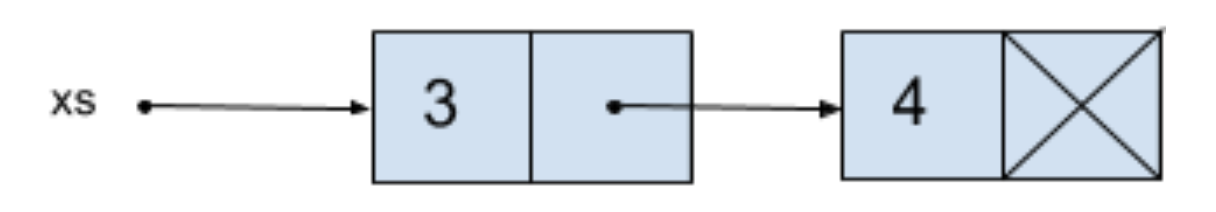
\includegraphics[width=0.5\textwidth]{../images/list34.png}

\end{footnotesize}
\end{frame}


\begin{frame}[fragile]
\begin{footnotesize}

  \head{Implementation of \lstinline{List.exists} med rekursion}

  \vspace{1ex}
  Vi kan afgøre om et element er i en liste ved hjælp af rekursion og brug af en prædikat-funktion:
\begin{lstlisting}[numbers=none,frame=none,mathescape]
let rec exists (p: 'a -> bool) (xs: 'a list) : bool =
  match xs with [] -> false
              | y :: ys -> p y || exists p ys

let b = exists (fun x -> x=23) [34;23;56]

// exists p [34;23;56] $\evals$
// p 34 || exists p [23;56] $\eval$ (34=23) || exists p [23;56] $\eval$
// false || exists p [23;56]  $\eval$ exists p [23;56] $\evals$
// p 23 || exists p [56] $\eval$ (23=23) || exists p [56] $\eval$
// true || exists p [56] $\eval$ true
\end{lstlisting}

\headsp{Bemærk:}

\begin{itemize}
\item Udtrykket \lstinline[mathescape]{$e_1$ || $e_2$} håndteres specielt i
  F\# (boolsk eller)!
\item Udtrykket $e_2$ evalueres kun hvis $e_1$ evaluerer til
\lstinline{false}.
\end{itemize}
\end{footnotesize}
\end{frame}

%%%%%%%%%%%%%%%%%%%%%%%%%%%%%%%%%%%%%%%%%%%%%%%%
\subsection{Rekursion over arrays}
%%%%%%%%%%%%%%%%%%%%%%%%%%%%%%%%%%%%%%%%%%%%%%%%

\begin{frame}[fragile]
\begin{footnotesize}

  \headsp{Binær søgning i sorteret array}

  Vi kan finde et heltal i et \textbf{sorteret} array hurtigere end ved at gennemløbe arrayet.

  \head{Binær søgning i array:}
\begin{lstlisting}[numbers=none,frame=none,mathescape]
let inSorted (arr:int[]) (x:int) : bool =
  let rec bs min max =
       if min > max then false
       else let mid = (max+min) / 2
            in if x < arr.[mid] then bs min (mid-1)
               else if x > arr.[mid] then bs (mid+1) max
               else true
  in bs 0 (Array.length arr - 1)

let arr = [|23;34;41;56;76;123;323;500|]  // sorteret array
do printf "%A\n" (inSorted arr 76)
\end{lstlisting}

\head{Kald af funktionen \lstinline{bs}:}
  \vspace{.5ex}
\begin{enumerate}
\item \lstinline{bs 0 7} $\eval$ \lstinline{mid} = 3
\item \lstinline{bs 4 7} $\eval$ \lstinline{mid} = 5  \hfill $\longleftarrow$ only $\id{log}(n)$ steps\ldots
\item \lstinline{bs 4 4} $\eval$ \lstinline{mid} = 4 $\eval$ \lstinline{true}
\end{enumerate}

\end{footnotesize}
\end{frame}

\subsection*{Konklusion}
\begin{frame}[fragile]
  \headsp{Konklusion}

  \vspace{3mm}
  \tableofcontents
\end{frame}


\end{document}
